\documentclass[11pt,a4paper]{article}
\usepackage[utf8]{inputenc}
\usepackage[english]{babel}

\usepackage{graphicx}
\usepackage[english]{babel}
\usepackage[margin=0.85in]{geometry}
\usepackage{amsmath}
\usepackage{natbib}
\usepackage{hyperref}
\bibliographystyle{plainnat}
\usepackage{setspace}


% These are the configurable settings
% Please change them to make it fit your course
\def \institute {Institute / project name}
\def \authors { Youri Hoogstrate, \institute }
\def \servers {
\begin{itemize}
	\item \url{https://usegalaxy.org/}
	\item \url{https://bioinf-galaxian.erasmusmc.nl/galaxy/}
\end{itemize}
}
\def \datalibrarydir {
	TraIT Galaxy Training Materials
		$\rightarrow$
	TraIT Galaxy Training - 1: Introduction to Galaxy
}

\begin{document}
\title{ \textit{\institute}\text{ }Galaxy Training: Introduction to Galaxy \\
{ \large This practical aims to familiarize you with the Galaxy user interface. It will teach you how to perform basic tasks such as uploading data, running tools, working with histories, creating workflows, and sharing data. } }

\author{ \authors }
\maketitle

%\newpage
%\tableofcontents
%\newpage

%\doublespacing

\section*{Introduction}
This manual is inspired by the Galaxy-101 pages available at \url{https://github.com/nekrut/galaxy/wiki/Galaxy101-1} and \url{https://usegalaxy.org/u/galaxyproject/p/galaxy-variant-101}.
Due to the rapid development of Galaxy screenshots and results may be out of date. If you experience something like this, please report it as a bug at \url{https://github.com/ErasmusMC-Bioinformatics/galaxy-courses/issues}.

% @todo -> make 1 genereric Preparations page and include it
% It should describe:
% - server address(es)
% - whether to use specific training accounts or register one
% - a notice until when the server will be available or whether it will be accessible after the course
% - funding related notices
\section*{Preparations}
\subsection*{Open Galaxy}
Please open a web browser and navigate to your assigned Galaxy server:

\servers

\subsection*{Register for an account}
In the top menu bar, go to User and then choose Register (fig. \ref{fig:registration}). After registration, click on Analyze data in the top menu to return to the main screen.

\begin{figure}
 \center
  
\includegraphics[scale=0.6]{figures/register_icon_1}
  \caption{\small{ The icons used in Galaxy to go to the registration page }}
  \label{fig:registration}
\end{figure}

\subsection*{Getting started}
The time is there to play with Galaxy. The main screen consists of three parts, on the left is the list of available tools, on the right side
is your history pane, showing the analysis you have performed so far, and in the middle you view your tools and data (fig. \ref{fig:organization_layout}).

\begin{figure}
 \center
  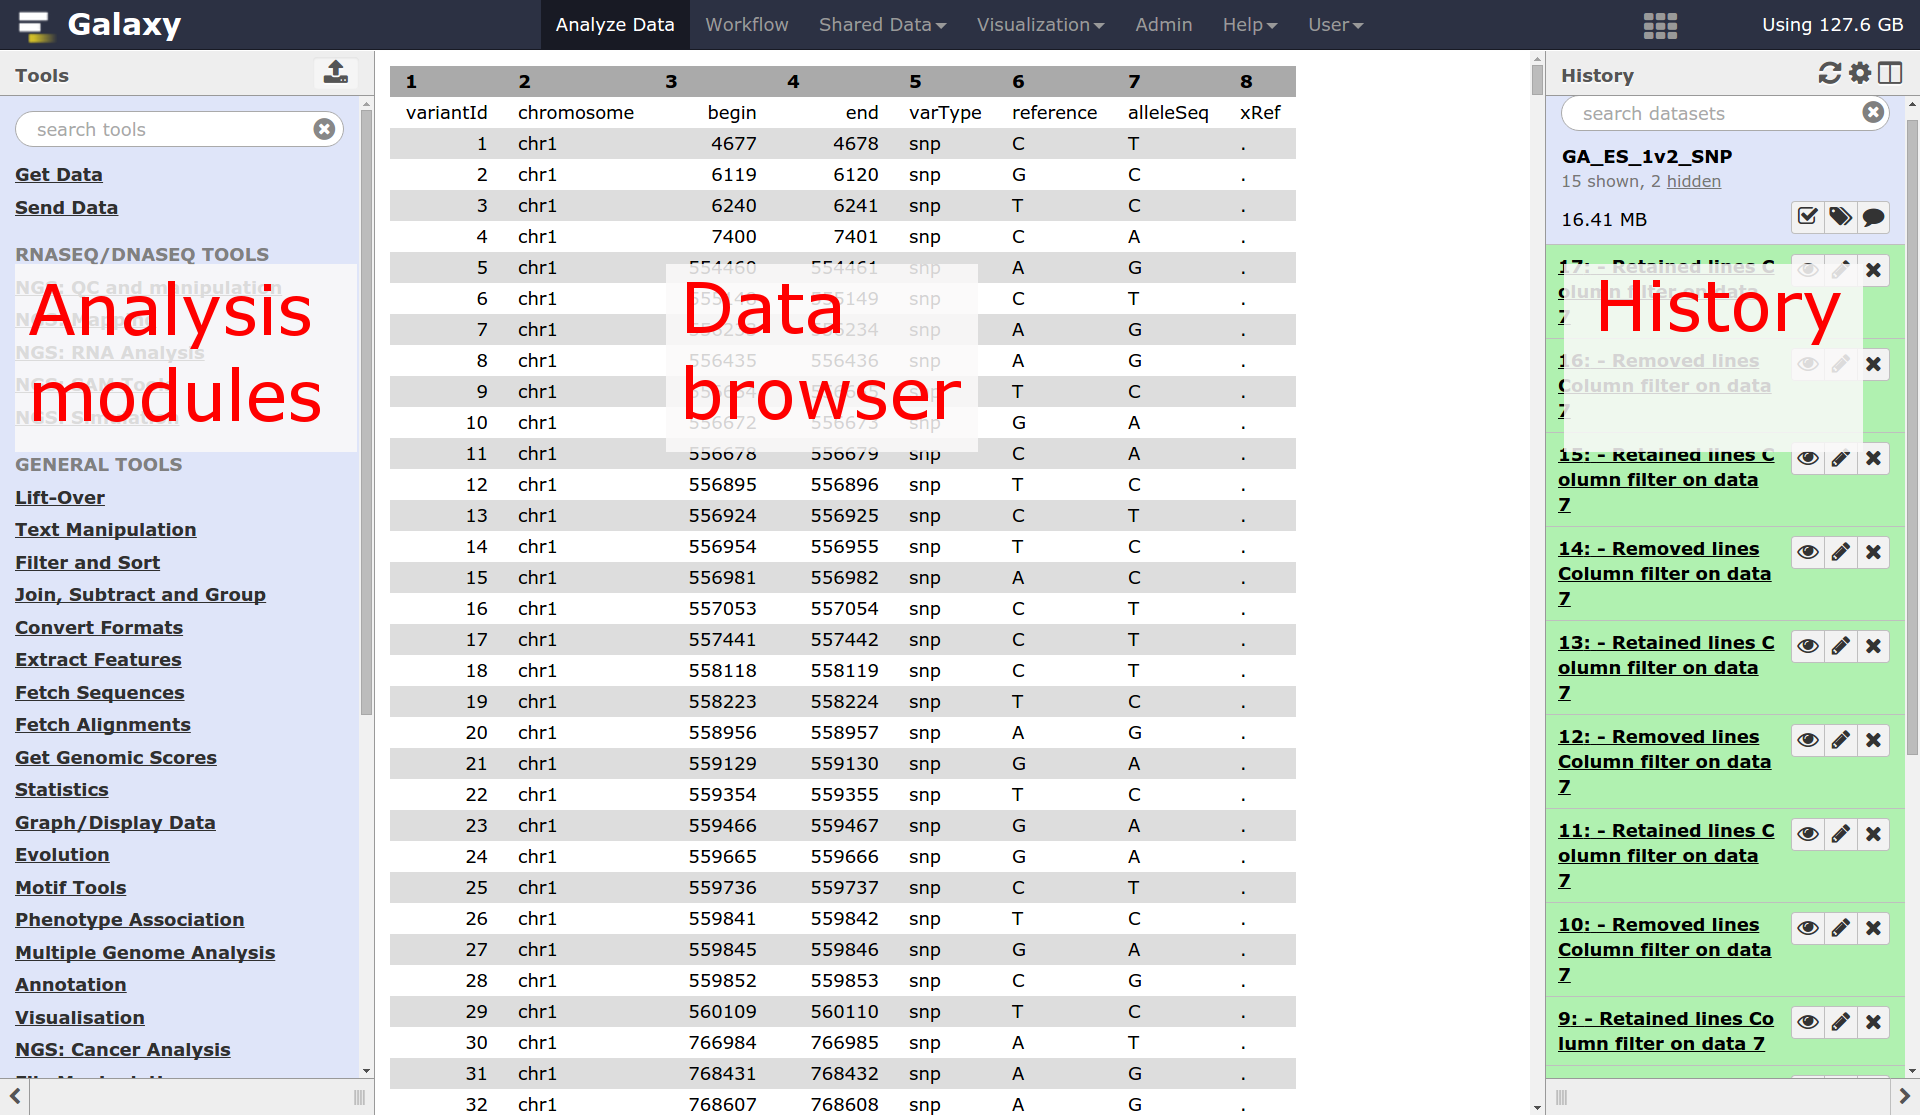
\includegraphics[width=\textwidth]{figures/galaxy_layout}
  \caption{\small{ The organization of Galaxy: on the left side the analysis modules like tools and workflows, in the middle page the data or the controls of the analysis modules, and on the right side the history items. }}
  \label{fig:organization_layout}
\end{figure}

\section*{Galaxy 101: The first thing you should try}
In this very simple example we will introduce you to bare basics of Galaxy:
\begin{itemize}
	\item Getting data from UCSC
	\item Performing simple data manipulation
	\item Understanding Galaxy's Tool and History system
	\item Creating and editing workflows
	\item Applying workflows to your data
\end{itemize}
Suppose you get the following question: ``\textit{Mom (or Dad) ... Which coding exon has the highest number of single nucleotide polymorphisms on chromosome 22?}''. You think to yourself ``\textit{Wow! This is a simple question ... I know exactly where the data is (at UCSC) but how do I actually compute this?}'' The truth is, there is really no
straightforward way of answering this question in a time frame comparable to the attention span of a 7-year-old. Well ... actually there is and it is called Galaxy. So let's try it...

\section{Getting data from UCSC genome browser}

First thing we will do is to obtain data from UCSC by clicking ``Get Data $\rightarrow$ UCSC Main'':\\
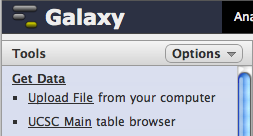
\includegraphics[scale=0.65]{figures/101_01} \\
You will see Galaxy's middle pane change to looks like this:\\
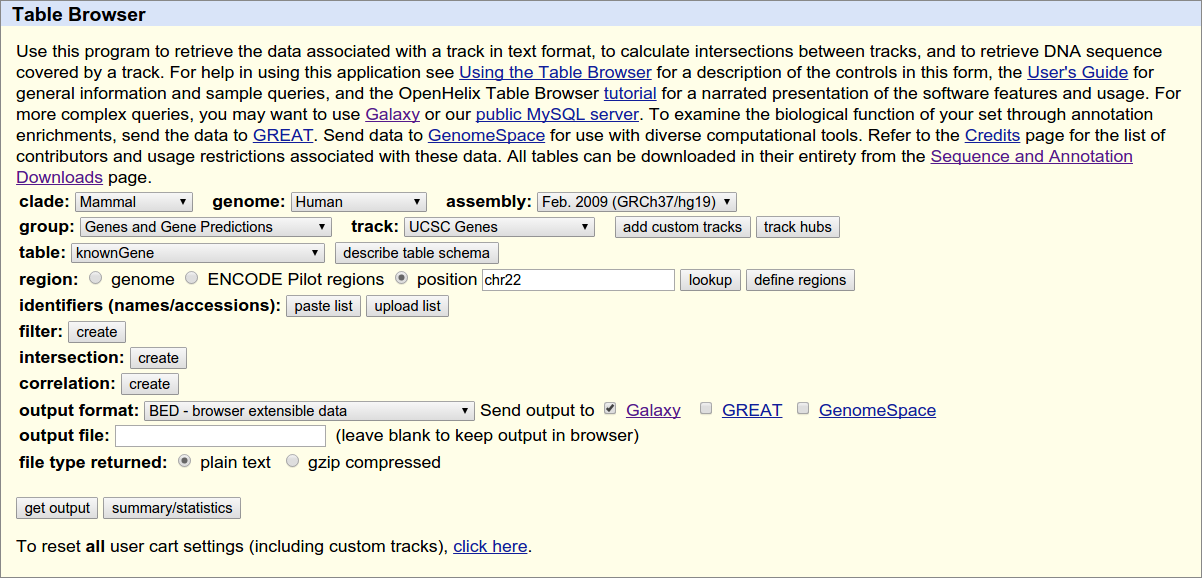
\includegraphics[width=\textwidth]{figures/101_02} \\
Make sure that your settings are exactly the same as shown on the screen (in particular, \textbf{assembly} should be set to \textit{Feb. 2009 (GRCh37/hg19}, \textbf{position} should be set to ``chr22'', \textbf{output format} should be set to ``BED - browser extensible data'', and ``Galaxy'' should be checked by Send output to option). Click get output and you will see the next screen:\\
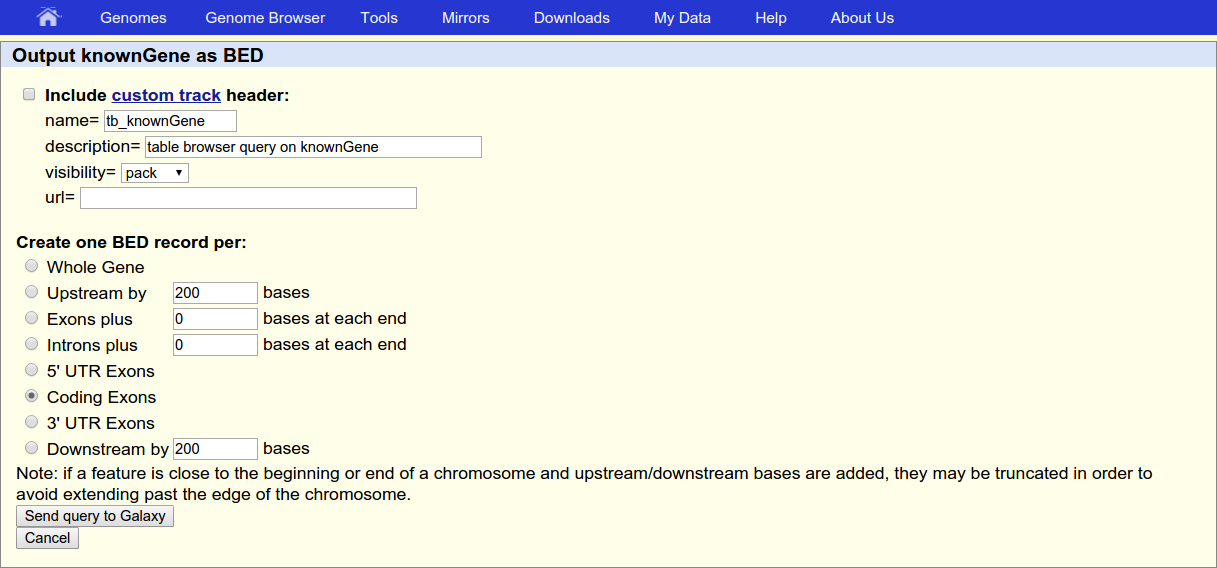
\includegraphics[width=\textwidth]{figures/101_03}\\
Make sure \textbf{Create one BED record per} is set to ``Coding Exons'' and click \textbf{Send Query to Galaxy}. After this you will see your first History Item in Galaxy's right pane. It will go through gray (preparing) and yellow (running) states to become green:\\
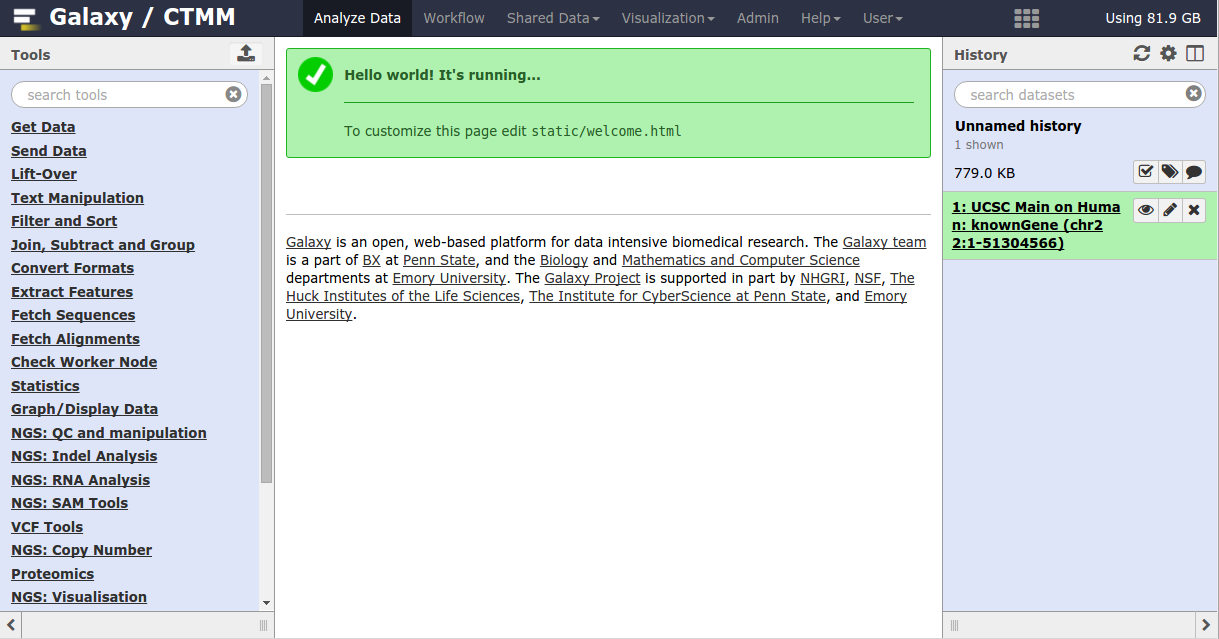
\includegraphics[width=\textwidth]{figures/101_04}\\
To view the contents of the file, click on the eye icon.

\subsection{Gettings SNPs}
Now is the time to obtain SNP data. This is done almost exactly the same way. First thing we will do is to again click on ``Get Data $\rightarrow$ UCSC Main'':\\
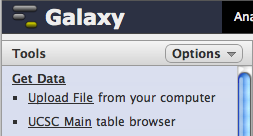
\includegraphics[scale=0.65]{figures/101_01}\\
But now change group to ``Variation'' to obtain the SNPs. It may be that newer versions of \textbf{Common SNPs ($\ldots$)} are available. It is not a big deal to select another one (if the one in the figure below is not available anymore), but the results will be slightly different. After selection the page will look like this:\\
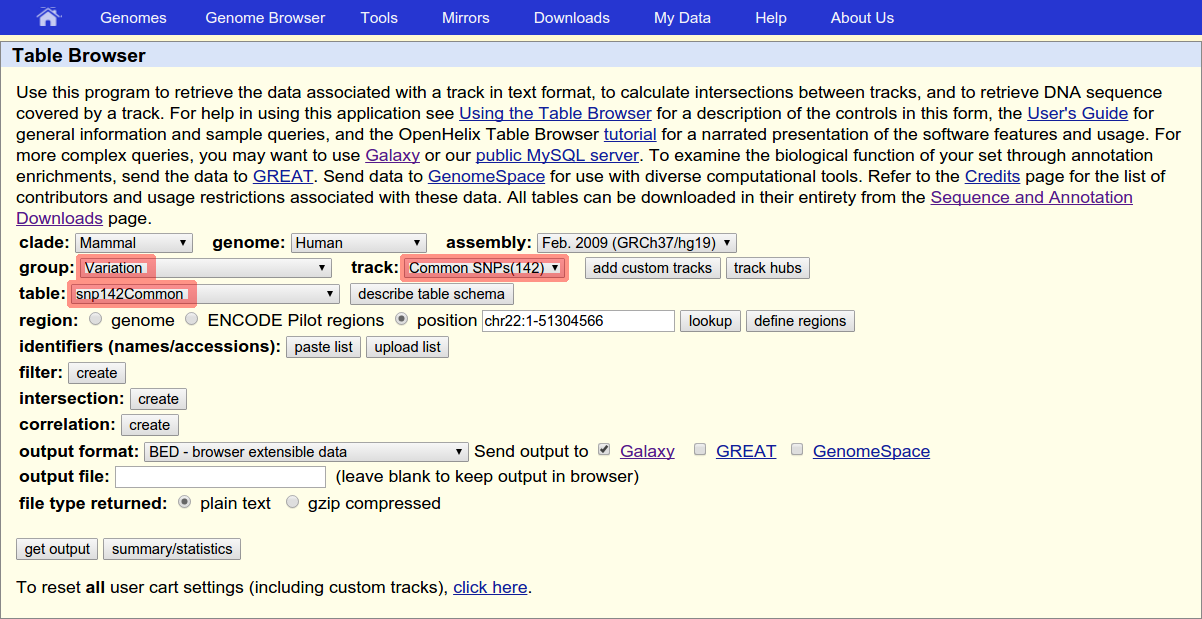
\includegraphics[width=\textwidth]{figures/101_06}\\
Then click \textbf{get output} to find a menu similar to this:\\
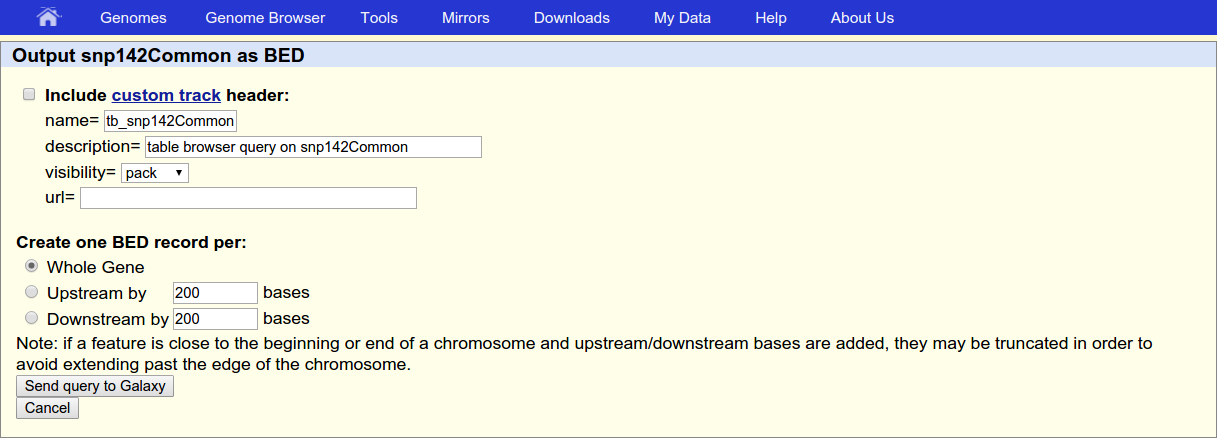
\includegraphics[width=\textwidth]{figures/101_07}\\
You need to make sure that \textbf{Whole Gene} is selected (``Whole Gene'' here really means ``Whole Feature'') and click \textbf{Send Query to Galaxy}. You will get your second item in the history:\\
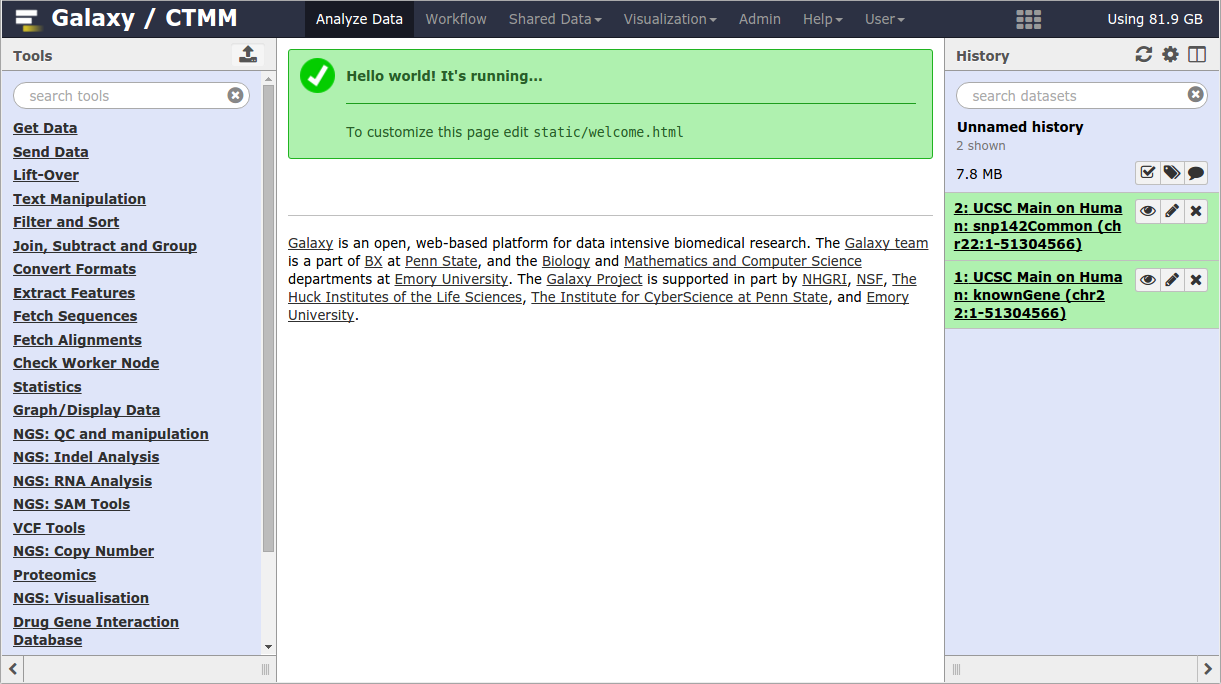
\includegraphics[width=\textwidth]{figures/101_08}\\
Now we will rename the two history items to ``Exons" and ``SNPs" by clicking on the Pencil icon adjacent to each item. Also we will rename history to "Galaxy 101" (or whatever you want) by clicking on "Unnamed history" so everything looks like this:\\
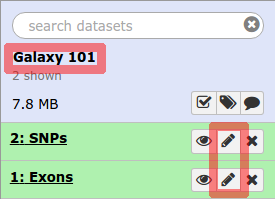
\includegraphics[scale=0.65]{figures/101_09}\\
\textbf{NOTE}: If the import from UCSC takes too long or something else went wrong, the files can still be found as shared data library in Galaxy. Browse the following directories \textit{
\datalibrarydir}
, and select the files named ``SNPs'' and ``Exons'', choose ``Import to current history'' and click ``Go''. Click on ``Analyze Data'' on the top menu bar to return to your analysis. In more recent versions of Galaxy you only have to ``to History". Go back to Galaxy's main page by pressing ``Analyze Data'':
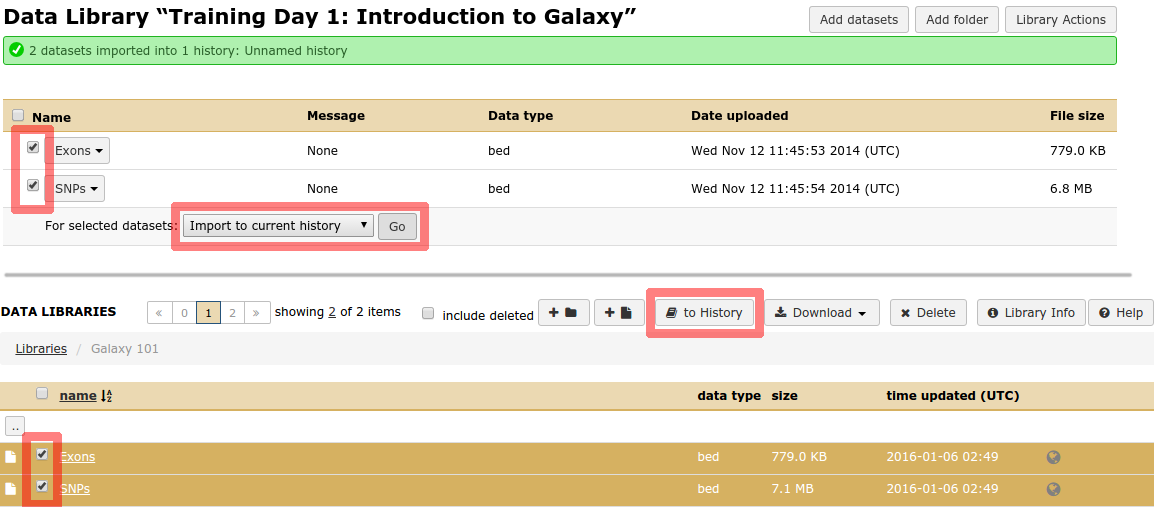
\includegraphics[width=\textwidth]{figures/101_10}\\



%\bibliographystyle{natbib}
%\bibliographystyle{plainnat}

\newpage

\vspace{-1.5em}
\bibliography{references}

\end{document}